\begin{figure*}
\centering{}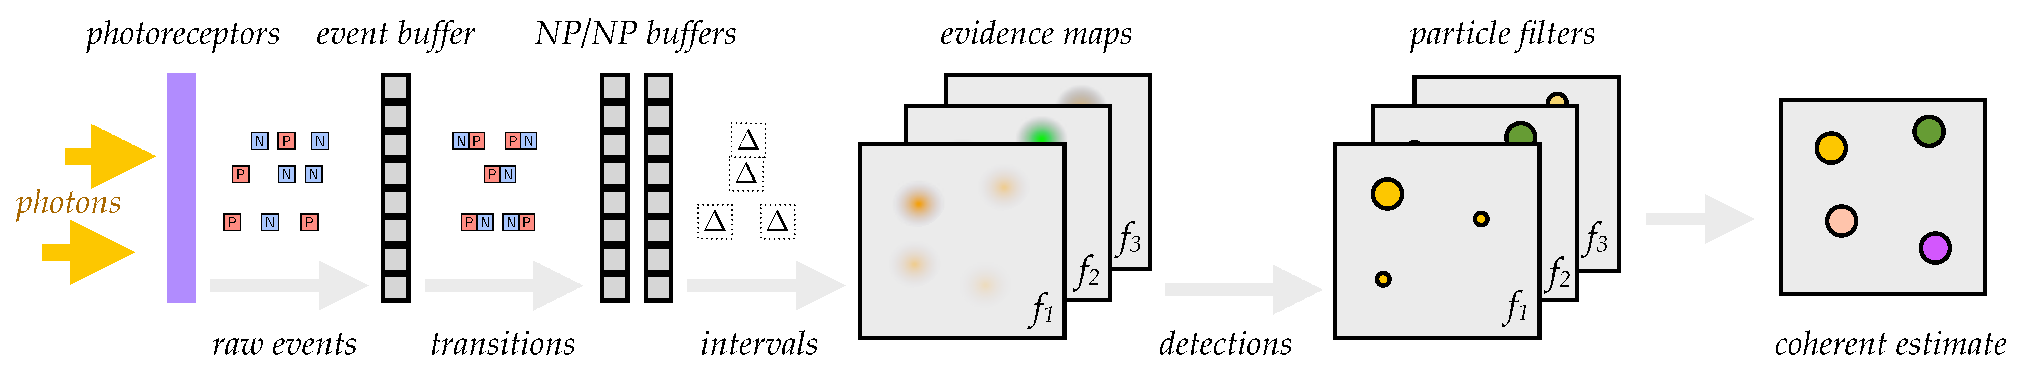
\includegraphics[width=16cm]{figures/slides/overall1}\caption{Our method proceeds in stages. We buffer the raw events, which have
either positive (\pP) or negative (\pN) polarity, as to find the
transitions, either positive-to-negative (\pPN) or negative-to-positive
(\pNP). Then, we look at the intervals $\Delta$ between two transitions
of the same type. These will be converted into votes in an evidence
map tuned to each frequency. From the evidence map we extract local
maxima, which are the instantaneous detections on where is each \ALM.
The rest of the method is standard: for each frequency we use a particle
filter to be robust to missed detections; then we choose the combination
of particles that gives a coherent global estimate for all \ALMs.}
\end{figure*}



\section{DVS-based Active LED Marker tracking }

This section describes our method for tracking the position of a set
of \ALMs from the output of a DVS. The input to the algorithm is
a sequence of events representing the change of luminance in a single
pixel. The output is an estimate of the pose of the quadrotor. We
describe the algorithm as a sequence of stages that process asynchronous
events; in principle, several of them could be implemented in hardware.

The webpage \xxx contains the source code of a C++ and a Python implementation.

\begin{figure}[H]
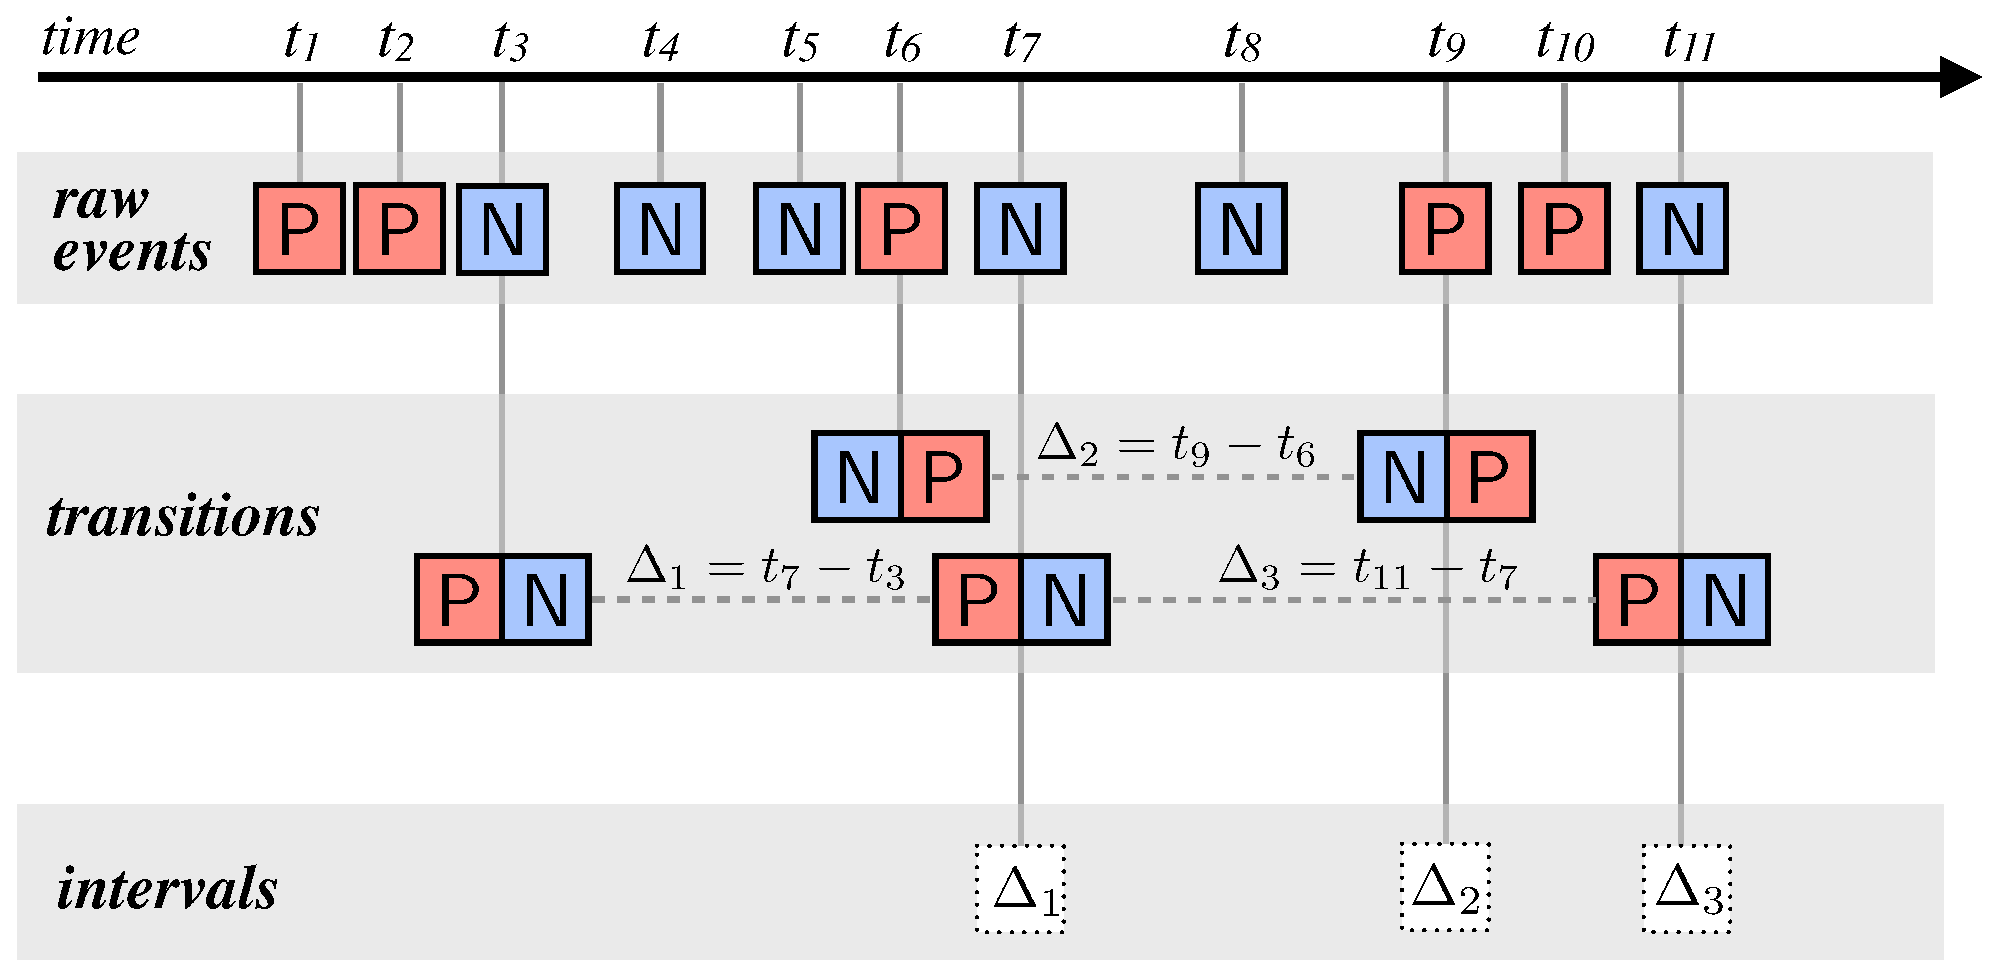
\includegraphics[width=8.6cm]{figures/slides/stages2}

\caption{A single pixel produces an irregular series of raw events, with polarity
either positive (\pP) or negative (\pN), each with its own timestamp.
The first stage of processing consists in looking for positive-to-negative
(\pPN) or negative-to-positive (\pNP) transitions. The second stage
consists at looking at two successive transitions of the same kind.
For example, two successive \pPN transitions at time $t_{3}$ and
$t_{7}$ generate an hyper-event with interval $\Delta=t_{7}-t_{3}$.
Assuming that these events are generated by a blinking \ALM, the
$\Delta$ is a good robust estimator of the blinking period.}
\end{figure}



\subsection{Raw events}

The input to the algorithm is the sequence of events in the address-event
representation (\xxx). Each event can be considered as a tuple 
\[
\langle t_{k},\: p_{k},\:\langle x_{k},y_{k}\rangle\rangle,
\]
where: 
\begin{itemize}
\item the scalar $t_{k}$ is the timestamp of the event generated; these
are not equispaced.
\item the value $p_{k}\in\{\pP,\pN\}$ is the \emph{polarity}, which is
either positive~(\pP) or negative~(\pN), according to whether
the luminance increased or decreased;
\item the coordinates $\left\langle x_{k},y_{k}\right\rangle \in\{0,\dots,127\}\times\{0,\dots,127\}$
identify the pixel that triggered the event.
\end{itemize}

\subsection{Transitions}

The first stage transforms the sequence of $\{\pP,\pN\}$ events into
a sequences of \emph{transition events} $\{\pPN,\pNP\}$. This stage
is independent for each pixel. Consider only the events that are produced
by a given pixel at coordinates $\left\langle x,y\right\rangle $.
At all times, we remember the last event timestamp $t_{k-1}$ and
the polarity $p_{k-1}\in\{\pP,\pN\}$. Every time the polarity of
the current event~$p_{k}$ is different than $p_{k-1}$, we create
a \emph{transition event}. If the polarity is the same, no transition
event is generated. This is described by the rules in \prettyref{tab:From-raw-events}. 

A transition event is a tuple 
\[
\langle t_{k},\: q_{k},\:\langle x_{k},y_{k}\rangle\rangle,
\]
where: 
\begin{itemize}
\item the scalar $t_{k}$ is the timestamp of the \emph{second} event that
triggered the transition.
\item the value $q_{k}\in\{\pP,\pN\}$ is the transition polarity, which
is either positive-to-negative~(\pPN) or negative-to-positive~(\pNP).
\item $\left\langle x_{k},y_{k}\right\rangle $ are the coordinates.
\end{itemize}
\begin{center}
\begin{table}[H]
\begin{centering}
\caption{\label{tab:From-raw-events}From raw events to transitions}

\par\end{centering}

\centering{}\normalsize %
\begin{tabular}{ccc}
\emph{last event} & \emph{current event} & \emph{transition event}\tabularnewline
\hline 
\multirow{2}{*}{$\langle t_{k-1},\ \pP,\:\langle x,y\rangle\rangle$} & $\langle t_{k},\ \pP,\:\langle x,y\rangle\rangle$ & none\tabularnewline
 & $\langle t_{k},\ \pN,\:\langle x,y\rangle\rangle$ & $\langle t_{k},\ \pPN,\:\langle x,y\rangle\rangle$\tabularnewline
\multirow{2}{*}{$\langle t_{k-1},\ \pN,\:\langle x,y\rangle\rangle$} & $\langle t_{k},\ \pP,\:\langle x,y\rangle\rangle$ & $\langle t_{k},\ \pNP,\:\langle x,y\rangle\rangle$\tabularnewline
 & $\langle t_{k},\ \pN,\:\langle x,y\rangle\rangle$ & none\tabularnewline
\end{tabular}
\end{table}

\par\end{center}


\subsection{Hyper-transitions}

The next stage of processing looks at the interval between successive
transitions of the same type. For each pixel, we remember the last
transition of either type (\pPN or \pNP) in a separate storage;
then, for each transition, we generate a ``hyper-transition'', which
is a tuple of the kind 
\[
\langle t_{k},\,\Delta_{k},\:\langle x_{k},y_{k}\rangle\rangle,
\]
where $\Delta_{k}$ is the interval between transitions of the same
kind, and $\langle x_{k},y_{k}\rangle$ are the coordinates. Note
that we dropped the polarity of the transitions, as they are not needed
in the following stages.


\subsection{Evidence maps}

We suppose to have been given a set of $n$ frequencies $\{f_{i}\}$,
$i\in\{1,n\}$ corresponding to the $n$ \ALMs to track. For each
frequency separately we construct an ``evidence map'' $I_{i}(\left\langle x,y\right\rangle ,t)$
over the visual field corresponding to the probability that the \ALM
is at that pixel. Each hyper-transition contributes to all evidence
maps, but with a different weight, so that we can integrate all information
and do not commit to saying that a given event belongs to the 

A hyper-transition with interval $\Delta_{k}$ contributes to the
evidence map of frequency $f_{i}$ with a weight that is proportional
to $p(\Delta_{k}\mid f_{i})$; that is, the likelihood that a marker
\ALM with that frequency produces a hyper-transition of that interval.
This distribution is found experimentally to be well approximated
by a Gaussian (see the data in \prettyref{fig:switch-hist}\emph{b},
which give $\sigma=30\ \mbox{Hz}$): 
\begin{equation}
p(\Delta_{k}\mid f_{i})=\mathcal{N}\left(\frac{1}{\Delta_{k}}-f_{i},\sigma^{2}\right).\label{eq:lik_delta}
\end{equation}
The evidence maps collect events within a time slice corresponding
to an interval of $1/f_{i}$. Therefore the value of the evidence
map $I_{i}(\left\langle x,y\right\rangle ,t)$ for a pixel $x,y$
and at time $t$ is given by the sum of the contributions of all events
at the given pixel and in the interval $\left[t-1/f_{i},t\right]$:
\[
I_{i}(\left\langle x,y\right\rangle ,t)=\sum_{t_{k}\in\left[t-\frac{1}{f_{i}},t\right]\wedge\left\langle x_{k},y_{k}\right\rangle =\left\langle x,y\right\rangle }\mathcal{N}\left(\frac{1}{\Delta_{k}}-f_{i},\sigma^{2}\right).
\]
To increase robustness at the expense of latency, it is also possible
to use multiples of the interval $1/f_{i}$ for the time slice.

At the end of the time slice, the evidence map $I_{i}(\left\langle x,y\right\rangle ,t)$
can be interpreted as the likelihood that the $i$-th \ALM with frequency
$f_{i}$ is at position $\left\langle x,y\right\rangle $. In our
experimental setting, this map is multimodal, with a strong peak at
the true position of the marker, and lower peaks at the positions
at the other markers, because each event contributes weakly, according
to~\prettyref{eq:lik_delta}, also to the evidence maps of the other
frequencies. 

We extract $m$ local maxima, at least $\delta$ pixels from each
other (in our experiments $m=3$, $\delta=15\,\mbox{px}$). The value
of the evidence map at the local maxima is used as a weight $w$ to
be carried forward to the next stage. The detections generated in
this way have a time $t$, coordinates $\left\langle x,y\right\rangle $
and the weight $w_{j}^{i}$: 
\[
\{\langle t,\,\langle x_{j}^{i},y_{j}^{i}\rangle,\, w_{j}^{i}\rangle\},\ j\in\{1,\dots,m\}.
\]



\subsection{Filtering }

Once we have these detections, the method proceeds in a conventional
way, as in any tracking problem, to achieve robustness to missed detections
and false alarms. 

First we use a particle filter to evolve particles for each frequency.
Each particle has coordinates $\langle x,y\rangle$, a weight~$w$
(carried over from the last step), as well as an isotropic spatial
uncertainty~$r$, which starts at $1\,\mbox{px}$. The uncertainty
grows using a motion model, which should be chosen according to how
on how fast things are predicted to move on the visual field. We have
computed that for the range of motions of a quadrotor, the maximum
apparent motion is approximately $1$ pixel/ms, which is quite slow
for the DVS.

We have a particle filter for each frequency. The particles in each
filter represent the posterior over the pose of one \ALM. To look
for a globally consistent solution, we choose the combination of particles
from all filters with the highest combined weight such that no two
markers can be too close to each other (in our experiments, $d=15$
pixels). 




\subsection{Pose reconstruction}

Assuming we have the position of the \ALMs in image space, and we
know the relative position of the markers in the world, we can reconstruct
the pose of the object using established techniques.
\begin{itemize}
\item \textbf{DS: one paragraph here }
\end{itemize}
\lorem
